\section{Zielsetzung}

Versuchsziel ist es, sich mit der Funktionsweise des Lock-In-Verstärkers vertraut zu machen. 
Außerdem soll für 10 verschiedene Phasen mit und ohne Störung die Funktionsweise verifiziert werden. 
Zuletzt soll die Rauschunterdrückung mit einer Photodetektorschaltung überprüft werden.

\section{Theorie}
\label{sec:Theorie}
Lock-In-Verstärker werden eingesetzt, um Signale mit hohem Rauschen zu messen. 
%Im Gegensatz zum Bandpass kann hier auch Rauschen herausgefiltert werden, welches auf der selben Frequenz wie das Messsignal liegt.
%
Das zu messende Eingangssignal $U_\mathup{sig}$ durchläuft im Gerät verschiedene Bauelemente, die in Abbildung \ref{fig:lockin} dargestellt sind.
\begin{figure}
	\centering
		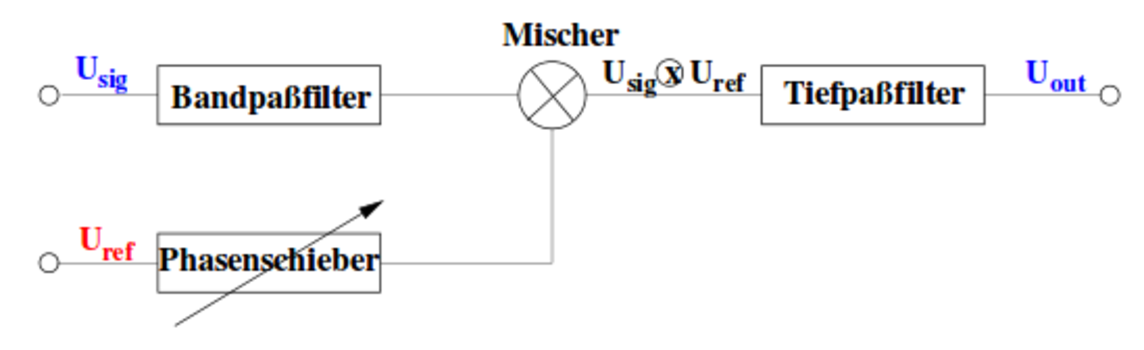
\includegraphics[width=0.7\textwidth]{Bilder/LOCK_IN.pdf}
		\caption{Schematischer Aufbau des Lock-In-Verstärkers. \cite{V303}}
		\label{fig:lockin}
	\end{figure}

Nach der Verstärkung durch den \emph{Pre-Amplifier} durchläuft das Signal zunächst einen \emph{Bandpassfilter}, der das Rauschen minimiert. 
Alle Frequenzen $\omega<<\omega_0$ und $\omega>>\omega_0$ werden grob herausgefiltert.
Ein \emph{Funktionsgenerator} erzeugt die Referenzspannung $U_\mathup{ref}$ -- eine Sinus- oder Rechteckspannung der Frequenz $\omega_0$ -- , welche über den \emph{Phasenschieber} an die Phase des Eingangssignals angepasst werden kann. 
Dieser Vorgang nennt sich Synchronisation.
Im \emph{Mischer} treffen beide Signale aufeinander und werden multipliziert. 
Anschließend wird das Mischsignal $U_\mathup{sig}\times U_\mathup{ref}$ an den \emph{Tiefpass} weitergeleitet, der die Modulationsfrequenz $\omega_0$ über mehrere Perioden integriert, um restliche Rauschanteile $\omega\neq\omega_0$ auszuschließen. 
Zurück bleiben nur die Anteile der Signalsspannung $U_\mathup{sig}$, die mit der Referenzspannung synchronisiert werden konnten.
Um eine möglichst geringe Bandbreite $\Delta{\nu}=\frac{1}{\pi RC}$ zu erhalten, sollte die Zeitkonstante $\uptau=RC$ des \emph{Tiefpasses} ausreichend groß gewählt werden. 
Damit wird eine hohe Güteziffer im Bezug auf Störungsfilterung erzielt.

Die Ausgangsspannung $U_\mathup{out}$ ist eine Gleichspannung, welche proportional zur Eingangsspannung $U_\mathup{sig}$ und zum Cosinus der Phasendifferenz $\Delta\Phi$ ist:
\begin{equation}
 	U_\mathup{out}\propto{U_\text{sig}}\text{cos}(\mathup{\Delta}\Phi). 
 	\label{cosinus_ausgangsspannung}
 \end{equation} 
$U_\mathup{out}$ wird also maximal, wenn die Phasendifferenz $\mathup{\Delta}\Phi=0°$ (wahlweise Vielfache von 180°) beträgt. \cite{regensburg}
%Quellenangabe http://www.physik.uni-regensburg.de/studium/praktika/a2/download/versuch5a.pdf

\begin{figure}
	\centering
		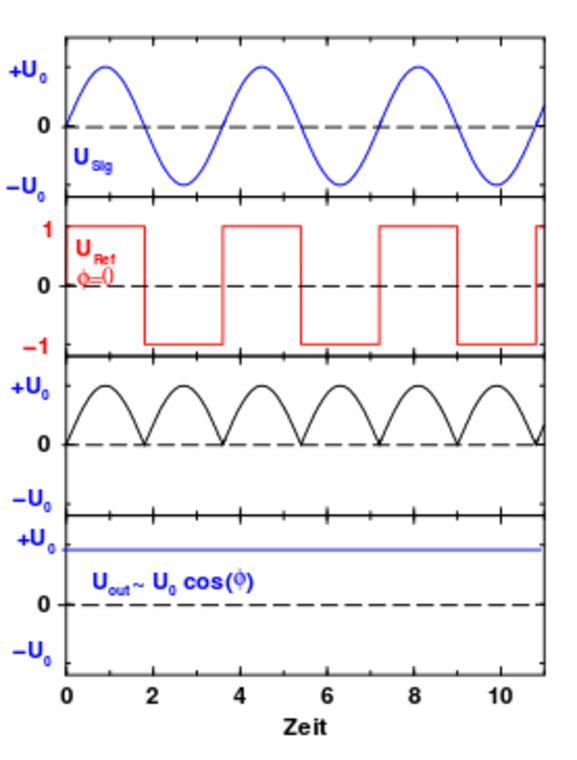
\includegraphics[width=0.4\textwidth]{Bilder/Beispiel.pdf}
		\caption{Überlagerung eines Sinus-förmigen Eingangssignals mit rechteckiger Referenzsspannung. \cite{V303}}
		\label{fig:bsp}
	\end{figure}
Wird beispielsweise ein Sinus-förmiges Eingangssignal $U_\mathup{sig}=U_0\text{sin}(\omega t)$ wie in Abbildung \ref{fig:bsp} mit einem rechteckigen Referenzsignal $U_\mathup{ref}$ gleicher Frequenz gefaltet, wird diese zunächst durch eine Fourierreihe angenähert, welche aus den ungeraden Harmonischen der Grundfrequenz besteht. 
Wird das multiplizierte Signal,  bestehend aus geraden Oberwellen der Frequenz $\omega$, durch den als Gleichrichter funktionierenden Tiefpass geleitet, ergibt sich die Endspannung
\begin{equation}
	U_\mathup{out}=\frac{2}{\pi}U_0\text{cos}(\mathup{\Delta}\Phi).
\end{equation}
Besteht kein Phasenunterschied zwischen Eingangs- und Referenzsignal, so nimmt die Endspannung ihren Maximalwert 
\begin{equation}
	U_\mathup{out}=\frac{2}{\pi}U_0
\end{equation}
an.
Die Rechteckspannung mit auf 1 genormten Amplitude realisiert einen Schalter (\enquote{Chopper}). 
Indem die Werte 1 und -1 durch positive und negative Halbwellen angenommen werden, steht der Schalter auf \enquote{Ein} bzw. \enquote{Aus}.



